% SC4023 --- Chapter 2: LLM Code Generation (0->100 ground-up)
\chapter{Code Generation with Large Language Models}
\label{ch:codegen}
\sloppy

\begin{quote}
\emph{``The best way to predict the future is to invent it.''} --- Alan Kay. Code-generating models try to do both at once: they predict the next token and thereby invent the program that follows your intent.
\end{quote}

\noindent\fbox{\parbox{\dimexpr\linewidth-2\fboxsep-2\fboxrule}{%
\textbf{From zero: no LLM background assumed.} We start from an empty file and a cursor: what does it mean to predict code, how does a model learn that skill from millions of repositories, and how do you talk to it so it helps rather than hallucinates? Every term---token, prompt, pass@$k$---is built picture-first, then defined.}}
\vspace{0.4em}

\section*{Learning Outcomes}
After this chapter you will be able to:
\begin{enumerate}[label=(L\arabic*)]
    \item explain how LLMs are trained on code (tokens, next-token loss, context window);
    \item craft prompts using zero-shot, few-shot, and chain-of-thought patterns;
    \item describe how GitHub Copilot turns cursor context into suggestions;
    \item compute \texttt{pass@$k$} on HumanEval and interpret what it measures;
    \item state failure modes (hallucination, leakage, insecurity) and mitigations.
\end{enumerate}

% ============================================================
\section{How a Model Learns to Write Code}
\label{sec:how-llm-code}
\paragraph{Intuition.} A junior developer learns by reading thousands of files: they see that after \texttt{for i in range(} the next characters are usually \texttt{len(arr))}, and after \texttt{def test\_} the next lines often assert something. An LLM learns the same regularities, but at scale---over billions of tokens---and stores them as weights that predict what comes next.

Formally, source code is split into \emph{tokens} (roughly words or subwords). Given a prefix $x_{1:t-1}$, the model learns a distribution $P_\theta(x_t \mid x_{1:t-1})$ and is trained to minimise \emph{cross-entropy} next-token loss on a large code corpus:
\[
\mathcal{L}(\theta) = -\sum_{t}\log P_\theta(x_t \mid x_{1:t-1}).
\]
A \emph{Transformer} implements $P_\theta$ with self-attention: each position attends to all previous positions, so the prediction for the next token sees the full prefix (prompt + file context + cursor). Pretraining on raw code gives a \emph{base model}; fine-tuning on prompt--response pairs (instruction tuning) and on accepted edits (RLHF or direct preference) steers it toward helpful completions.

\begin{figure}[h]\centering
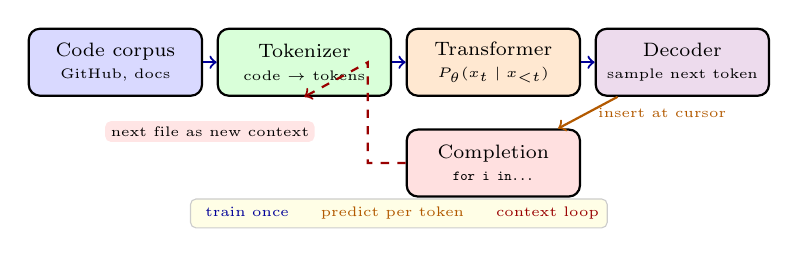
\begin{tikzpicture}[scale=0.80,every node/.style={font=\scriptsize},
  box/.style={draw,thick,rounded corners=4pt,minimum width=2.2cm,minimum height=0.85cm,align=center}]
  \node[box,fill=blue!15] (corp) at (0,0) {Code corpus\\\tiny GitHub, docs};
  \node[box,fill=green!15] (tok) at (3.0,0) {Tokenizer\\\tiny code $\to$ tokens};
  \node[box,fill=orange!18] (trans) at (6.0,0) {Transformer\\\tiny $P_\theta(x_t\mid x_{<t})$};
  \node[box,fill=violet!14] (dec) at (9.0,0) {Decoder\\\tiny sample next token};
  \node[box,fill=red!12] (comp) at (6.0,-1.6) {Completion\\\tiny \texttt{for i in...}};
  \foreach \a/\b in {corp/tok,tok/trans,trans/dec}
    \draw[->,thick,blue!60!black] (\a) -- (\b);
  \draw[->,thick,orange!70!black] (dec) -- (comp) node[midway,right,font=\tiny] {insert at cursor};
  \draw[->,thick,red!60!black,dashed] (comp.west) -- ++(-0.6,0) -- ++(0,1.6) -- (tok.south);
  \node[font=\tiny,fill=red!10,rounded corners=2pt,inner sep=2pt] at (1.5,-1.1) {next file as new context};
  \node[font=\tiny,align=left,fill=yellow!10,draw=gray!40,rounded corners=2pt,inner sep=3pt] at (4.5,-2.4) {\textcolor{blue!60!black}{$\blacksquare$ train once} \quad \textcolor{orange!70!black}{$\blacksquare$ predict per token} \quad \textcolor{red!60!black}{$\blacksquare$ context loop}};
\end{tikzpicture}
\caption{LLM for code as next-token prediction. Training minimises $-\log P_\theta$ over a tokenised corpus; at inference the model samples tokens one by one conditioned on the prompt and surrounding file context.}
\label{fig:llm-pipeline}
\end{figure}

Two limits matter immediately. The \emph{context window} (e.g., 8k--128k tokens) caps how much surrounding code the model can see; beyond it, information is truncated. \emph{Exposure bias} means training sees ground-truth prefixes but generation feeds its own past samples, so errors can compound.

\begin{example}[Next-token intuition]
Prefix: \texttt{def fib(n):\textbackslash n\ \ \ \ if n <= 1:\textbackslash n\ \ \ \ \ \ \ \ }. The model assigns high probability to \texttt{return n} and to \texttt{return 1}, lower to \texttt{print(}. Sampling picks one; temperature controls how adventurous the pick is.
\end{example}

% ============================================================
\section{Prompting: Talking to the Model}
\label{sec:prompting}
\paragraph{Intuition.} A prompt is not a magic spell; it is a specification written in natural language plus examples. The same model can produce insecure, correct, or over-engineered code depending on how you frame the request. Prompt engineering is specification engineering with a probabilistic interpreter.

Three patterns cover most uses. \emph{Zero-shot}: describe the task outright (``Write a Python function that returns the median of a list''). \emph{Few-shot}: give 2--3 input--output examples before the real request, anchoring style and edge cases. \emph{Chain-of-thought (CoT)}: ask the model to reason step by step before coding (``First list edge cases, then write the function''); this often reduces off-by-one and null-handling errors.

\begin{lstlisting}[language=Python, caption={Three prompting styles for the same task. The code is the same; the prompt changes the result.}, label={lst:prompting}]
# Zero-shot: bare instruction
# Prompt: "Write a Python function median(xs) that handles empty and even-length lists."
def median_zero_shot(xs):
    if not xs: return None
    s = sorted(xs); n = len(s)
    return s[n//2] if n % 2 == 1 else (s[n//2-1]+s[n//2])/2

# Few-shot: show examples, then the task (model imitates pattern)
# Example 1: median([3]) -> 3   Example 2: median([1,2,3,4]) -> 2.5
# Now complete: median([5,1,9]) -> ?

# Chain-of-thought prompt (in comment) -> model writes reasoning first
# "Steps: 1) handle empty, 2) sort, 3) if odd return middle else average two middles."
def median_cot(xs):
    # step 1: empty guard
    if not xs: return None
    # step 2: sort
    s = sorted(xs); n = len(s); mid = n//2
    # step 3: branch on parity
    return float(s[mid]) if n % 2 == 1 else (s[mid-1]+s[mid])/2.0
\end{lstlisting}

Practical tips: be explicit about language, I/O format, and edge cases; include a tiny example when the output shape matters; forbid unwanted behaviour (``do not use recursion''); and ask for tests alongside code. The model is sensitive to all of these.

\paragraph{Prompt sensitivity.} Small rewordings can swing correctness: adding ``handle empty input'' may fix a null failure; swapping the order of examples may change which edge case the model copies. This brittleness is not a bug to patch but a property of probabilistic models: the prompt is the specification, and vague specifications yield variable implementations. Good prompts are precise, minimal, and testable.

\begin{definition}[Prompt as specification]
A \emph{prompt} is a (possibly incomplete) specification of the desired program in natural language plus optional examples and constraints. Better prompts reduce the set of programs consistent with the specification, but they never reduce it to one---the model still samples.
\end{definition}

% ============================================================
\section{GitHub Copilot in Practice}
\label{sec:copilot}
In the IDE, Copilot sees far more than your prompt: the open file, neighbouring files, cursor position, and recent edits. It ranks candidate completions by model score and by heuristics (how well they parse, whether they reuse identifiers in scope). The developer's job shifts from writing every character to \emph{reviewing} candidates---accept, edit, or dismiss.

\begin{figure}[h]\centering
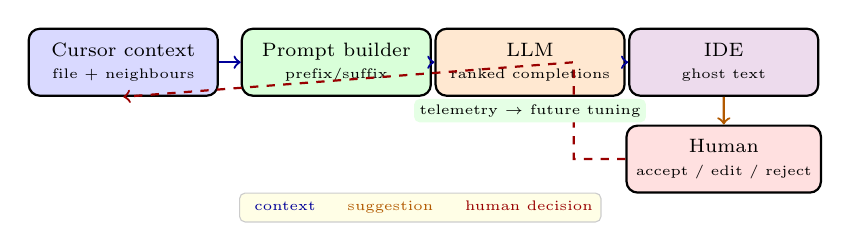
\begin{tikzpicture}[scale=0.82,every node/.style={font=\scriptsize},
  box/.style={draw,thick,rounded corners=4pt,minimum width=2.4cm,minimum height=0.85cm,align=center}]
  \node[box,fill=blue!15] (ctx) at (0,0) {Cursor context\\\tiny file + neighbours};
  \node[box,fill=green!15] (prompt) at (3.3,0) {Prompt builder\\\tiny prefix/suffix};
  \node[box,fill=orange!18] (llm) at (6.3,0) {LLM\\\tiny ranked completions};
  \node[box,fill=violet!14] (ide) at (9.3,0) {IDE\\\tiny ghost text};
  \node[box,fill=red!12] (human) at (9.3,-1.5) {Human\\\tiny accept / edit / reject};
  \foreach \a/\b in {ctx/prompt,prompt/llm,llm/ide}
    \draw[->,thick,blue!60!black] (\a) -- (\b);
  \draw[->,thick,orange!70!black] (ide) -- (human);
  \draw[->,thick,red!60!black,dashed] (human.west) -- ++(-0.8,0) -- ++(0,1.5) -- (ctx.south);
  \node[font=\tiny,fill=green!10,rounded corners=2pt,inner sep=2pt] at (6.3,-0.75) {telemetry $\to$ future tuning};
  \node[font=\tiny,align=left,fill=yellow!10,draw=gray!40,rounded corners=2pt,inner sep=3pt] at (4.6,-2.25) {\textcolor{blue!60!black}{$\blacksquare$ context} \quad \textcolor{orange!70!black}{$\blacksquare$ suggestion} \quad \textcolor{red!60!black}{$\blacksquare$ human decision}};
\end{tikzpicture}
\caption{Copilot's inline loop. Context is turned into a prompt, the model proposes ranked completions rendered as ghost text, and the developer decides. Telemetry (accept/reject/edit) later tunes ranking.}
\label{fig:copilot-loop}
\end{figure}

Empirical studies report 30--55\% acceptance rates for shown completions and measurable speed-ups on boilerplate and test scaffolding, with smaller gains on novel algorithmic code. The risk is not just wrong code but \emph{plausible} wrong code---it type-checks, looks idiomatic, and fails on an edge case the prompt omitted.

% ============================================================
\section{Evaluation: HumanEval and What It Misses}
\label{sec:humaneval}
\paragraph{Intuition.} To know whether a model is useful, you need a test where the answer is unambiguous. HumanEval provides that: 164 hand-written Python problems, each with a function signature, docstring, and hidden unit tests. The model generates code; we run the tests; it either passes or not.

The metric is \emph{pass@$k$}: generate $k$ samples per problem, count the problem as solved if \emph{any} sample passes all tests. For $n$ samples with $c$ correct, the unbiased estimator used in practice is
\[
\text{pass@}k = 1 - \frac{\binom{n-c}{k}}{\binom{n}{k}},\qquad
\text{and pass@1 is just accuracy when }k=1.
\]
Reporting pass@1, pass@10, and pass@100 shows the trade-off between single-try reliability and the value of re-sampling.

\begin{figure}[h]\centering
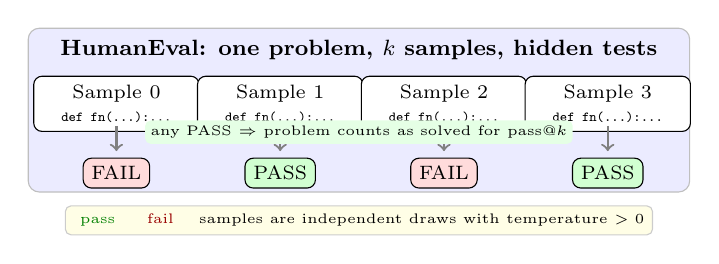
\begin{tikzpicture}[scale=0.80,every node/.style={font=\scriptsize}]
  \draw[fill=blue!8,draw=gray!50,rounded corners=4pt] (0,0) rectangle (10.5,2.6);
  \node[font=\footnotesize\bfseries] at (5.25,2.25) {HumanEval: one problem, $k$ samples, hidden tests};
  \foreach \i in {0,1,2,3} {
    \node[draw,fill=white,rounded corners=3pt,minimum width=2.1cm,minimum height=0.7cm,align=center] at (1.4+2.6*\i,1.4) {Sample \i\\\tiny \texttt{def fn(...):...}};
    \draw[->,thick,gray] (1.4+2.6*\i,1.05) -- (1.4+2.6*\i,0.65);
    \ifnum\i=1
      \node[draw,fill=green!18,rounded corners=3pt,inner sep=3pt] at (1.4+2.6*\i,0.30) {PASS};
    \else\ifnum\i=3
      \node[draw,fill=green!18,rounded corners=3pt,inner sep=3pt] at (1.4+2.6*\i,0.30) {PASS};
    \else
      \node[draw,fill=red!14,rounded corners=3pt,inner sep=3pt] at (1.4+2.6*\i,0.30) {FAIL};
    \fi\fi
  }
  \node[font=\tiny,fill=green!10,rounded corners=2pt,inner sep=2pt] at (5.25,0.95) {any PASS $\Rightarrow$ problem counts as solved for pass@$k$};
  \node[font=\tiny,align=left,fill=yellow!10,draw=gray!40,rounded corners=2pt,inner sep=3pt] at (5.25,-0.45) {\textcolor{green!50!black}{$\blacksquare$ pass} \quad \textcolor{red!60!black}{$\blacksquare$ fail} \quad samples are independent draws with temperature $>0$};
\end{tikzpicture}
\caption{Computing pass@$k$. Generate $k$ candidates per problem; the problem is solved if at least one candidate passes all hidden tests. Higher $k$ rewards diversity, not just single-shot precision.}
\label{fig:humaneval}
\end{figure}

\begin{lstlisting}[language=Python, caption={A HumanEval-style problem: the model must complete the function to pass hidden tests.}, label={lst:humaneval-ex}]
def has_close_elements(numbers, threshold):
    """Check if any two numbers are closer than threshold."""
    # Model must generate the body below to pass hidden tests
    for i in range(len(numbers)):
        for j in range(i+1, len(numbers)):
            if abs(numbers[i] - numbers[j]) < threshold:
                return True
    return False

# Hidden tests (not shown to model):
assert has_close_elements([1.0, 2.0, 3.0], 0.5) == False
assert has_close_elements([1.0, 2.8, 3.0], 0.3) == True
# pass@k: does any of k samples pass all asserts?
\end{lstlisting}

HumanEval is clean but narrow: single-function Python, no project context, no dependency on other files. Real utility needs broader suites---MBPP, DS-1000, SWE-Bench (full repository issues), and project-specific acceptance tests. Leakage (training data containing the benchmark) and prompt sensitivity further qualify any headline number.

\paragraph{Failure modes to watch.} Three recur in practice. \emph{Hallucination}: the model invents an API that does not exist (e.g., \texttt{df.to\_csv\_with\_header()}) with confident syntax. \emph{Insecurity}: it reproduces an unsafe pattern seen in training, such as string-interpolated SQL. \emph{Non-determinism}: the same prompt yields different outputs across runs (controlled by temperature); a completion that passed yesterday may fail today. Mitigations are engineering, not hopes: pin dependencies, run tests on every suggestion, and treat generated code as untrusted input.

\begin{definition}[Temperature]
\emph{Temperature} $T>0$ scales logits before softmax: lower $T$ sharpens the distribution (more deterministic, more typical), higher $T$ flattens it (more diverse, more surprising). For code, $T\approx0.2$ favours pass@1; $T\approx0.8$ favours pass@100 by trading precision for coverage.
\end{definition}

\begin{remark}[From benchmark to IDE]
A 10-point gain in pass@1 does not guarantee a 10\% productivity gain. Measure what you ship: acceptance rate, time to task, defect rate, and review comments. The benchmark tells you the model can code; your repository tells you whether it helps you code.
\end{remark}

% ============================================================
\section{Chapter Notes}
Chen et~al.\ (2021, Codex/HumanEval) introduced pass@$k$ and the 164-problem HumanEval set; Austin et~al.\ (MBPP) and Lai et~al.\ (DS-1000) broaden it. GitHub's Copilot reports and Ziegler et~al.\ (2022) study acceptance and productivity. For prompting, see Wei et~al.\ on chain-of-thought and recent code-specific prompt surveys. Security caveat: Pearce et~al.\ (2022) show language models can reproduce vulnerable patterns; always test and scan generated code.

% ============================================================
\section{Exercises}
\label{sec:ch02-exercises}
\begin{enumerate}[label=E2.\arabic*, leftmargin=*, itemsep=0.7em]
    \item \textbf{Tokens and context.} Tokenise \texttt{for i in range(len(xs)):} by hand into plausible tokens. If the model's context window is 8 tokens and your file prefix is 20 tokens long, which tokens are dropped and why might that cause a wrong completion for a variable defined at the top of the file?
    \item \textbf{Prompt design.} Write zero-shot, few-shot (2 examples), and chain-of-thought prompts for: ``Return the $k$ most frequent words in a text, case-insensitive, tie-broken alphabetically.'' Run all three on the same model (any public LLM) and compare outputs on an empty string and on ties.
    \item \textbf{pass@$k$ calculation.} For one HumanEval problem you draw $n=10$ samples and $c=3$ pass. Compute pass@1, pass@2, and pass@5 using the formula in \S\ref{sec:humaneval}. Explain why pass@10 would be $1.0$ in this setting and what that reveals about the metric.
    \item \textbf{Copilot loop.} Sketch the data that Copilot sends as context when your cursor is inside a function that calls an internal API \texttt{db.query(sql)}. What could go wrong if a secret appears in a neighbouring file? Propose one mitigation at the prompt-building stage and one at the review stage.
    \item \textbf{Beyond HumanEval.} A model scores 72\% pass@1 on HumanEval but only 18\% on SWE-Bench (repository-level issues). Give three concrete reasons for the gap that are not ``the model got worse.'' Propose one evaluation you would run on your own codebase before adopting the model.
\end{enumerate}
% End of Chapter 2
